

\chapterquote{We can only measure what Nature sends us}{Jim Cronin}  

Desde el descubrimiento de los rayos cósmicos en 1911 por Victor Hess, numerosos experimentos han intentado caracterizarlos. A partir del 2004, el Observatorio Pierre Auger ha detectado rayos cósmicos con el objetivo de estudiar su origen. Un análisis adecuado de los eventos registrados es necesario para estudiar las posibles fuentes de rayos cósmicos, además de su composición y su espectro de energía.

Un aspecto estudiado por varios trabajos \cite{collaboration2013pierre} \cite{data} es la distribución  de las direcciones de arribo de los rayos cósmicos. Las direcciones de arribo son prácticamente isotrópicas salvo variaciones muy pequeñas alrededor de la media. Dado que estas  anisotropías son pequeñas respecto a la media, es importante tener en cuenta todos los efectos que pueden ser fuentes de modulación de los datos. Un ejemplo claro de una modulación física que no aporta información sobre las anisotropías es la modulación del clima.

Este trabajo es parte del análisis de la direcciones de arribo de los rayos cósmicos de ultra alta energía obtenidas por el Observatorio Pierre Auger. En el mismo se estudia la modulación del clima sobre la determinación de la energía de los eventos medidos por los detectores de superficie. Las lluvias atmosféricas provocadas por los rayos cósmicos que llegan a la alta atmósfera, interactúan con los constituyentes de las atmósfera. Esta interacción puede ser afectada por los cambios en las condiciones atmosféricas en el momento de la lluvia. El trabajo está dividido en distintos capítulos organizados para introducir las rayos cósmicos, mencionar brevemente características del Observatorio Pierre Auger y presentar el análisis sobre la modulación del clima de la señal medida por el Observatorio.

\section{Rayos cósmicos}

Los rayos cósmicos (CRs) fueron descubiertos en el 1911 por Victor Hess \cite{hess1912}. Los mismos son partículas que llegan a la Tierra desde el espacio como  electrones, positrones, rayos gamma entre otros, además de núcleos atómicos. En 1962, John Linsley detectó un evento de CR con una energía de  $10^{20}\,$EeV, y otros experimentos  encontraron más eventos por encima de esta energía. A pesar de que han sido medidos y estudiados en experimentos alrededor del mundo, el origen de los CRs es incierto. Las partículas con energía por encima de $10^{18}\,$EeV se conocen como rayos cósmicos de ultra alta energía (UHECRs) y son las partículas con más energía presentes en el universo. Las direcciones de arribo de los UHECRs son casi isotrópicas  \cite{collaboration2013pierre} \cite{data} y se cree que son de origen extra-galáctico, es decir que no fueron producidos dentro de la Vía Láctea, debido a que los campos magnéticos galácticos no pueden confinarlos y la distribución de sus direcciones de arribo es cerca a ser isotrópica, sin correlación significativa con el plano o el centro galáctico. Para estudiar a los mismos, se disponen de tres observables principales: el espectro, la composición y la anisotropía. El espectro se refiere a la distribución de energía de los rayos cósmicos detectados, la composición es la distribución de masas nucleares, es decir, que elementos y en que proporción se encuentran en los rayos cósmicos y el tercero, la anisotropía, es la distribución de las direcciones de arribo a diferentes energías.

\section{Espectro de energías}

Los mecanismos de interacción de protones y núcleos de origen extra-galáctico  y su relevancia en la propagación fueron predichos por Greisen \cite{greisen1966end}, e independientemente por Zatsepin y Kuzmin \cite{zatsepin1966upper} tras el descubrimiento de la radiación cósmica de fondo (CMB). Primeramente todas las partículas sufren una pérdida de energía debido a la expansión del universo. Este el principal mecanismo de pérdida de energía para protones de $E < 2\times 10^{18}\,$eV y núcleos de $E/A < 0.5\times 10^{18}\,$eV. 

En la Fig.\,\ref{fig:spectra} se presenta el espectro de los rayos cósmicos medidos por los distintos experimentos que se desarrollaron para su estudio. La figura fue extraída de \cite{PGD}, donde los datos fueron multiplicado por $E^{2.6}$ para resaltar los cambios en la forma del espectro. Considerando que el espectro de energías por debajo de $\sim 0.1\times 10^{18}\,$eV es de origen galáctico, la rodilla correspondiente al cambio de pendiente en $\sim 3\times10^{15}\,$EeV podría reflejar el hecho que la mayoría de los aceleradores en la galaxia han alcanzado su energía máxima para la aceleración de protones. El experimento de Kascade-Grande ha reportado una segunda rodilla cercana a $8\times10^{16}\,$eV, que podría corresponder al límite de aceleración de primarios más pesados \cite{PGD}.

Considerando el tobillo en la Fig\,\ref{fig:spectra}, es posible que sea el resultado de que una población de mayor energía esté sobrepasando a una población de menor energía, por ejemplo un flujo extra-galáctico empiece a dominar sobre un flujo galáctico \cite{bird1994cosmic}. Otra posibilidad es que el cambio de la forma de la curva se deba a la pérdida de energía de los protones extra-galácticos, debido por el proceso $p\,\gamma \rightarrow\,e^+\,+\,e^-$, conocido como foto-desintegración con el CMB \cite{berezinsky2006astrophysical}. Para energías aun mayores ($\nicefrac{E}{A} \geq 60\times 10^{18}\,$eV ) el proceso dominante es la producción de mesones por colisiones entre núcleos y fotones de muy altas energías. 

El flujo de los rayos cósmicos en función de la energía puede aproximar una ley de potencias que tiene una forma del siguiente tipo
\begin{equation}
	    \frac{d\Phi_{CR}}{dE} \propto \ E^{-\gamma}   \label{eq:expresion1}
\end{equation}
donde $\gamma$ se lo denomina índice espectral, este valor varía ligeramente para distintos rangos de energía. %Para este trabajo se toma un valor de $\gamma = 3.29$ \cite{como_funciona_auger}. Este valor es un promedio de los distintos valores del índice espectral para UHCRs.

%\section{Desarrollo del primario desde su fuente hasta la cascada}

\section{Lluvias atmosféricas extendidas}

Una lluvia atmosférica extendida (EAS) es la cascada de partículas secundarias generadas por la interacción de un rayo cósmico, conocido como partícula primaria o el primario, con la atmósfera terrestre. Como se observa en la Fig.\,\ref{fig:spectra} el flujo de partículas decae rápidamente con la energía. Aunque para energías mayores a $10^{14}\,$EeV las partículas producidas en la atmósfera como secundarios pueden llegar a las montañas. Para energías mayores pueden llegar hasta el nivel del mar. El momento transversal que adquieren las partículas secundarias en el proceso de dispersión a través de la atmósfera es tal que los secundarios se dispersan sobre área de gran tamaño. Para energía mayores a 10$\,$EeV, por ejemplo, la lluvia puede llegar a cubrir más de 25\,km$^2$. 

El desarrollo de la lluvia puede describirse mediante la profundidad atmosférica, definida como la masa de aire por unidad de área que atravesó una partícula en su dirección de propagación, 
\begin{equation}
	X(L)= \int_L^\infty dx \rho(x)
\end{equation}
donde $\rho$ es la densidad del aire en función de la posición.


\section{Descripción de una anisotropía dipolar}
Las anisotropías en las direcciones de llegada de los RCs indican que ciertas zonas del cielo tienen una variación significativa con respecto a la media de flujo de RCs. Estas anisotropías pueden describirse mediante una superposición de funciones armónicas. El primer orden corresponde a una anisotropía dipolar.

\begin{figure}[H]
	\centering
	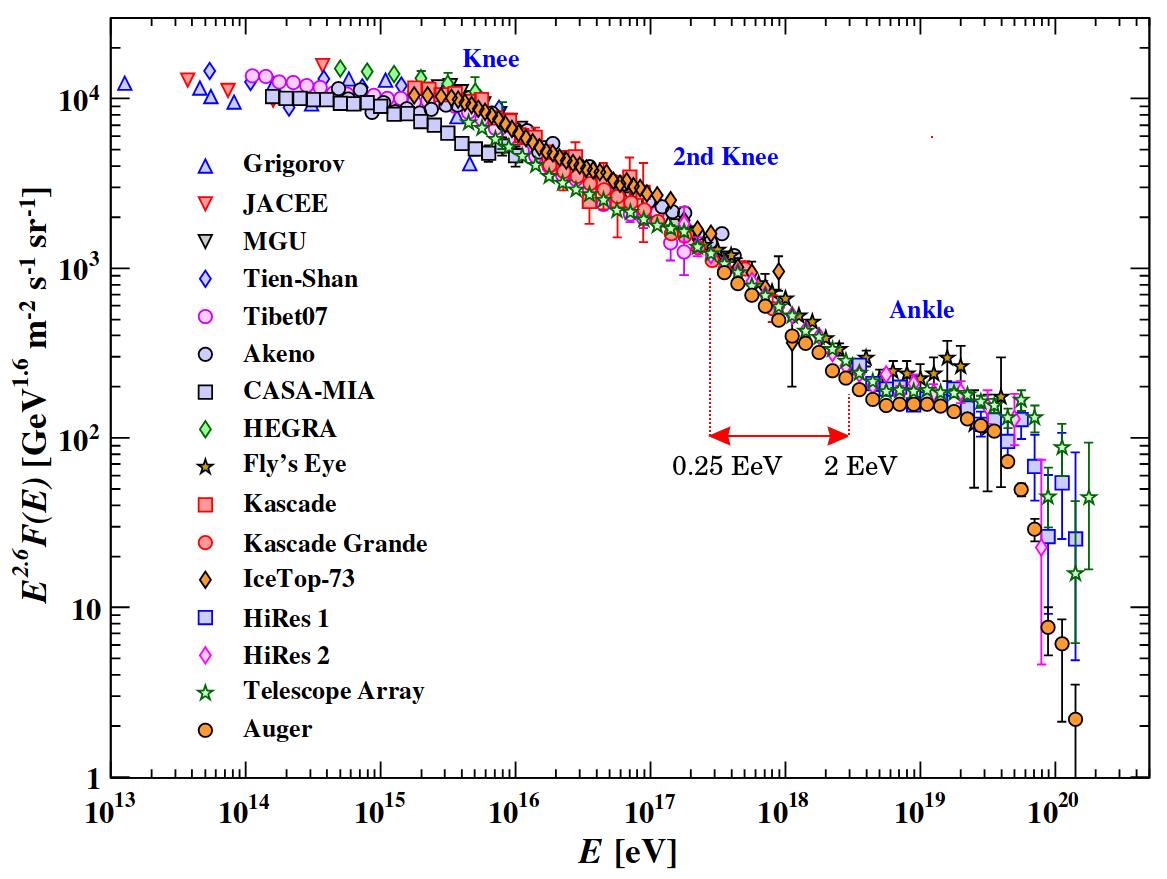
\includegraphics[width=0.7\textwidth]{auger_spectrum_v2.png}
	\caption{Espectro de rayos cósmicos medidos mediante lluvias atmosféricas en función de la energía $E$. Figura extraída de \cite{PGD}}
	\label{fig:spectra}
\end{figure}


Una anisotropía dipolar se puede describir de la siguiente forma:
\begin{equation}
    \Phi(\hat{\bf{u}}) = \Phi_0(1+\bf{d}\cdot\hat{\bf{u}})
    \label{eq:dipolo_general}
\end{equation}
\noindent donde $\Phi_0$ es el flujo medio de eventos, $\hat{\bf{u}}$ es un versor que apunta a la dirección a estudiar, y $\bf{d}$ es un vector con módulo igual a la amplitud del dipolo y cuya dirección está apuntando al máximo del flujo. Tomando coordenadas ecuatoriales \footnote{El sistema de coordenadas ecuatoriales se desarrolla en el apéndice \ref{apendice:ecuatorial}}, la dirección de $\bf{d}$ es $(\alpha_d, \delta_d$) y de $\hat{\bf{u}}$ es $(\alpha, \delta)$, entonces  el producto escalar  entre estos vectores se puede escribir de la siguiente manera:
\begin{equation}
    \textbf{d}\cdot\hat{\bf{u}}= d (\cos\delta_d \cos\delta \cos(\alpha - \alpha_d) + \sin\delta_d  \sin\delta)
    \label{eq:product_ud}
\end{equation}
El desarrollo para obtener esta expresión se encuentra en el apéndice \ref{cambio_coord}.

Otro aspecto importante de la representación del dipolo en coordenadas ecuatoriales, es que la proyección de la amplitud del dipolo sobre el plano ecuatorial $d_\perp$ se puede aproximar de la siguiente manera \cite{taborda} :
\begin{equation}
    d_\perp \simeq \frac{r_1}{ \langle \cos\delta \rangle}
    \label{eq:fourier_perp}
\end{equation}
donde $r_1$ es la amplitud del primer armónico en ascensión recta, y $\langle \cos\delta \rangle$ es el valor medio de $\cos\delta $ de los eventos.

\subsection{Representación en coordenadas locales de la anisotropía dipolar}

Podemos reescribir el producto escalar entre el dipolo $\textbf{d}$ y el versor $\hat{u}$ que apunta en una dirección cualquiera mediante las coordenadas locales $\theta$ y $\phi$\footnote{El sistema de coordenadas locales se desarrolla en el apéndice \ref{apendice:local}.} como se muestra en la siguiente expresión: 
\begin{align}
    \textbf{d} &=  d_{x'}(\alpha^0, \delta^0)\hat{x}' +  d_{y'}(\alpha^0, \delta^0)\hat{y}'+ d_{z'}(\alpha^0, \delta^0)\hat{z}' \\
    \hat{\bf{u}} &=\sin\theta \cos\phi \hat{x}' + \sin\theta \sin\phi \hat{y}' + \cos\theta\hat{z}'\\
    \textbf{d}\cdot\hat{\bf{u}} &= d_{x'}(\alpha^0, \delta^0)\sin\theta \cos\phi
    + d_{y'}(\alpha^0, \delta^0) \sin\theta \sin\phi  
     + d_{z'}(\alpha^0, \delta^0)\cos\theta \label{eq:dot-prod-local}
\end{align}
donde los versores $\hat{x}'$, $\hat{y}'$ y $\hat{z}'$ apuntan a la dirección Este, Norte y del cenit respectivamente. 

El dipolo $\textbf{d}$ está fijo en el cielo pero visto desde las coordenadas locales, para poder trabajar con $\theta$ y $\phi$, sus proyecciones  $d_{x'}$, $d_{y'}$ y $d_{z'}$ tienen una dependencia con la ascensión recta  $\alpha^0$ y declinación $\delta^0$ del cenit. 
